\documentclass[parskip=full]{scrartcl}
\usepackage[utf8]{inputenc} % use utf8 file encoding for TeX sources
\usepackage[T1]{fontenc}    % avoid garbled Unicode text in pdf
\usepackage[english]{babel}  % english hyphenation, quotes, etc
\usepackage[colorlinks=true,linkcolor=blue]{hyperref}       % detailed hyperlink/pdf configuration
\usepackage{graphicx}       % provides commands for including figures
\usepackage{csquotes}       % provides \enquote{} macro for "quotes"
\usepackage{enumitem}
\usepackage{multicol}
\setlength{\columnsep}{4cm}
%\usepackage{lscape}	% provides landscape portrait

\usepackage{pdflscape}	% provides horizental landscape portrait


\usepackage{pdfpages}	% add another pdf in  Latex

\usepackage{tikz}


\usepackage{verbatim}	% provides multi-line comments

\usepackage{afterpage}
\usepackage{ragged2e}
\usepackage[export]{adjustbox}
\newcommand\tab[1][1cm]{\hspace*{#1}}


\title{\Huge \textbf{HePICS Implementation Document}}
\date{\today \vspace{+10ex}}
\author{Andres Stober \\
	\and Mehyar Cherni \\
	\and Ibrahim Bouriga \\ 
	\and Linjuan Fan \\
	\and Bahaa Mahjane \\ }

\begin{document}

\maketitle
\thispagestyle{empty}

\begin{tikzpicture}[remember picture, overlay]
  \node [anchor=north west, inner sep=0.5pt, yshift=-20pt,xshift=20pt]  at (current page.north west)
     {
\includegraphics[height=1.9cm]{Logo_KIT}};
\end{tikzpicture}

\begin{figure}[b]
\centering
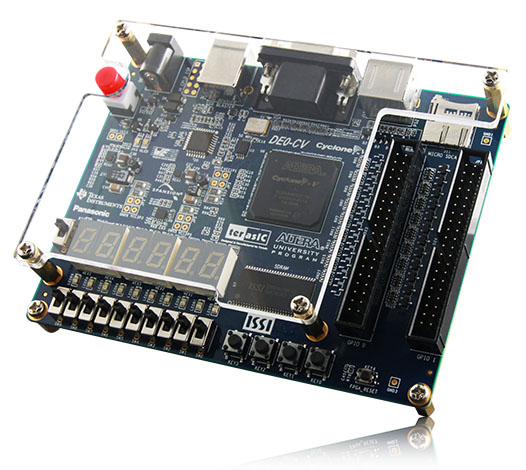
\includegraphics[width=0.45\textwidth, center]{boardimage}
\end{figure}

\pagebreak

\tableofcontents
\thispagestyle{empty}
\pagebreak



\section {Introduction}
	\tab In this document you will find a full description of the work flow in the implementation phase as well as the deviations and changes made on the class digaram. Those changes are sometimes necessary and have convincing reasons that will be mentioned in details.
	\subsection{Workflow}
	\tab In order to distribute tasks and maintain good communication between team members, we use a scrum framework online 	\url{https://app.vivifyscrum.com} and a github repository \url{https://github.com/Turon42/hepics}.
	
	\subsection{Tasks}
	\tab The project can be devided in six parts:
	\tab \begin{itemize}
	\item GUI \ref{GUI}
	\item Image and Neural Network Model  \ref{Image and Neural Network Model}
	\item Sheduler \ref{Scheduler}
	\item Connecting PFGA \ref{Connecting FPGA}
	\item Operation Modes  \ref{Operation Modes}
	\end{itemize}
	
\section{GUI} \label{GUI}
	@Linjuan Fan \textit{(No description provided yet)}
	\begin{center}
		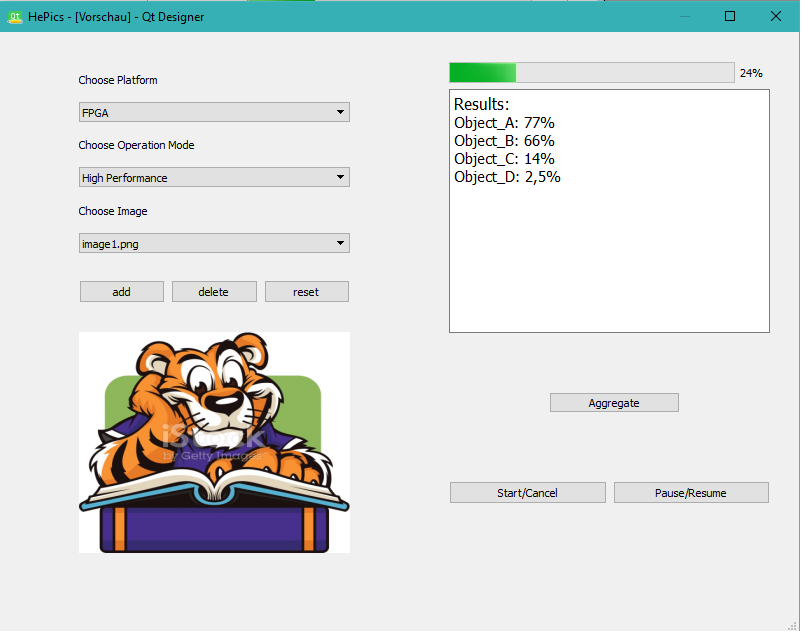
\includegraphics[width=0.9\textwidth]{NewMainWindow}
	\end{center}


\pagebreak

\section {Image and Neural Network Model} \label{Image and Neural Network Model}
	@Ibrahim Bouriga
	
	\subsection {Image Model}
	\tab The Image Class represents the \textbf{input} as well as the \textbf{filter} used in the different layers.\\
	The Image Manager Class however was removed in the implementation because all of its methods can be fully implemented as static ones in the Image Class.\\ As a result the use of this methods does not require any new instance object to be created and thus makes less use of memory. \\ Classes InputImage and ResultImage were not needed as results are only to display as text for the moment, as for input images, they are simply represented as instances of the class Image.\\ Here a list of of static methods implemented in Image:
	\begin {itemize}
		\item load\_image\_color: load an image
		\item load\_image: load an image an resize it if necessary
		\item load\_image\_stb: uses an external library to load an image. See \ref{External Libraries}
	\end{itemize}
	\subsection {Image and Result Saving}
	@Mehyar Cherni
	\tab The class #DataSaver is meant to work as a data base, it consists of one map whose keys are images' unique identifications #id, and whose values are results, represented as well as a an object. DataSaver allows the program to store input images and their results, retrieve them, delete them, or change their values. It also offers the possibility of saving the results of one classification in a text file. \\The aggregate function stores all classnames and percentages in a new map named #global, converts the map into a vector to sort it, then chooses the 4 biggest values and returns them as a #Result object.
\\The class #Result wasn't included in the design, and was added for the purpose of making the storage clearer and more flexible. It is meant to represent the results of a classification of a single input image as follows. Each instance of the object Result contains a map, that stores classnames represented as strings, and links them to their values stored as floats. Functionalities included are saving a classname and its percentage into the map. To control the number of classnames needed, we added the int i who counts the number of elements which are currently saved. This class offers the possibility to write results as plain text to display it on the GUI as such, classname1 : percentage1, classname2 : percentage2 etc ... 
	\subsubsection {Assistant}
	\tab Class #ClassificationAssistant has been renamed into Assistant. It serves the purpose of providing and storing all data given by the user through the GUI to the system. The weight file is loaded directly into the network through a configuration file, so it doesn't belong to the assistant anymore. The boolean function is classified has been removed since it hasn't been needed. The classnames file is set in the assistant, which will then be able to load them into a list of strings. Input images are stored into a list as well, with the possibility of deleting them by selection, or clearing the whole list.

	\subsection {Network Model}
	\tab The Network Model consists of the network and the layers:
	
		\subsubsection {Network}
		\tab The Network Class was implemented as it was introduced in the class diagram. However displaying the topology was not part of the implementation due to the fact that only the alexnet architecture will be deployed in the classification process. To display the topology of the neural network, an image whose path has been set from the beginning is displayed, in order to give an idea about the structure of the implemented neural network.
		The architecure (See \ref{fig:alexnet-architecture}) itself was described in a comprehensible configuration file, which will be parsed (See Parser \ref{Parser}) to extract relevant informations about the network.
		
		\subsubsection {Layer}
		\tab The Layer Class stores informations such as the number of inputs and outputs as well as the layer type and define the forward function which is implemented by derived classes:\\
		\begin{itemize}
			\item Convolutional Layer
			\item Max Pool Layer
			\item Connected Layer
			\item Softmax Layer
		\end{itemize}
		\begin{figure}
			\centering
			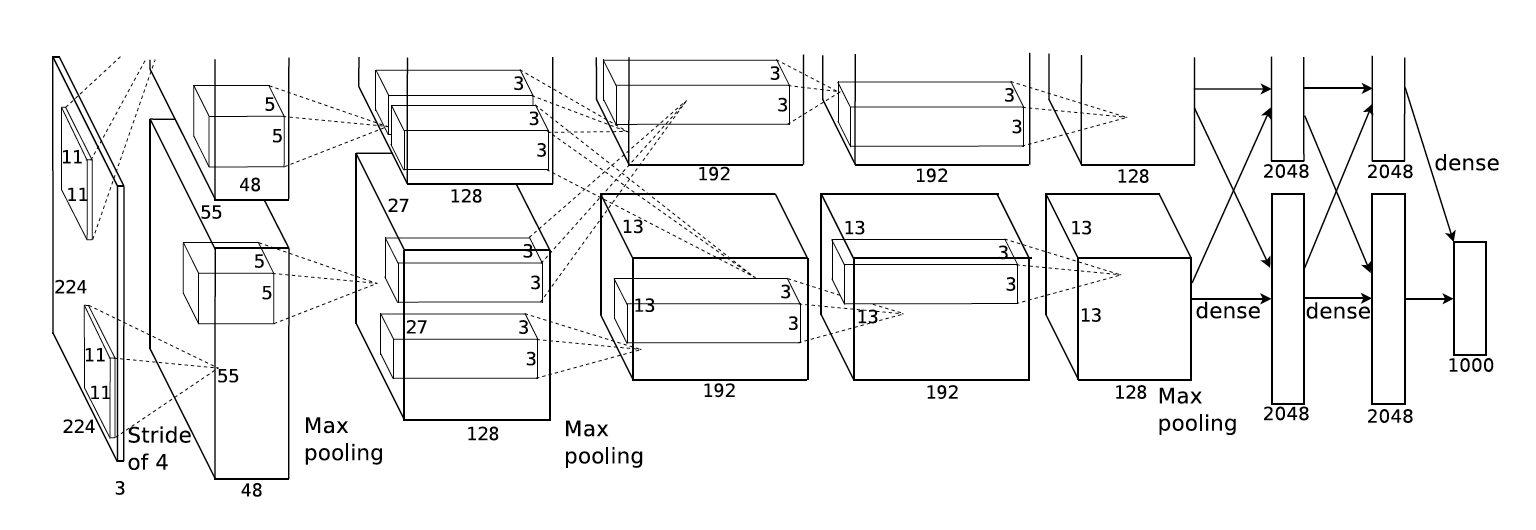
\includegraphics[width=1.0\textwidth]{alexnet-architecture}
			\caption{alexnet architecture}
			\label{fig:alexnet-architecture}
		\end{figure}
		
		\subsubsection {Activation}
		\tab The Activation Class implements the following activations functions:
		\begin{itemize}
			\item ReLu $g(z) = max{0, z}$
			\item Linear $g(z) =z$
			\item Tanh  $g(z) = (e^z -e^{-z}) / (e^z + e^{-z})$
			\item Sigmoid $g(z) = 1 / (1 + e^{-z})$
		\end{itemize}
		
	\subsection {New Classes}
		\paragraph{a.Parser} \label{Parser}
		\tab This class was created to parse and extract informations related to the network from the alexnet architecture (See \ref{fig:alexnet_architecture}).
		\begin{itemize}
			\item parse\_convolutional: create a convolutional layer from the convolution section in the configuration file
			\item parse\_maxpool: create a maxpool layer from the convolution section in the configuration file
			\item parse\_connected: create a connected layer from the convolution section in the configuration file
			\item parse\_softmax: create a softmax layer from the convolution section in the configuration file
			\item load\_network: create the network and initialize layers
		\end{itemize}
		
		\paragraph{b.Utils}
		\tab This class implements static methods that does logically not belong to any object. For instance file and memory errors. 
		
		\paragraph{c.Options\_list}
		\tab This class read datas from the configuration file line by line.\\
		It models a hash set with key words and associated values. The extracted values will be stored in lists (See \ref{Structures})
		
	\subsection {External Libraries} \label{External Libraries}
		\begin{itemize}
			\item stb\_image
			\item GEMM
			\item BLAS
			\item IM2COL
		\end{itemize}
		
	\subsection{Structures} \label{Structures}
		\tab Some availabe structures were implemented again in order to avoid unexpected behaviour like:
		\begin{itemize}
			\item List
			\item Node
		\end{itemize} 
		
\pagebreak

\section{Scheduler} \label{Scheduler}
	@Mehyar Cherni
	\tab Class #Scheduler has been set for the service of enabling and selecting the platforms corresponding to the selected mode. Following this logic, an enumeration type has been defined under the name Platform { 
	\begin {itemize}
		\item cpu, 
		\item gpu, 
		\item fpga
	\end{itemize}
	}. The class also consists of two other vectors of booleans. The first, named platforms, represents the platforms that the user has chosen to enable. The second, named use_platforms, defines which platforms are to run the code on, but only after the user chooses the operating mode. The choice of the use of platforms follows a comparison of the three platforms on three different levels, supposing that the code is meant to run parallel and contains mainly vector operations. 
	\begin {itemize}
		\item Power Consumption : cpu>gpu>fpga
		\item Performance : fpga>gpu>cpu
		\item Energy Efficiency : fpga>cpu>gpu
	\end{itemize}
\\ Next to accessing information about the mode and currently enabled/used platforms, #Scheduler also contains a vector of workers, whose size has to be defined while creating an instance of the class. Each worker can be assigned to execute a task on a selected platform, which he would only do if, this platform is allowed to use after the choosing process. \\A group of methods has been also made available for a possibly future parallel implementation of the classification.
	\begin {itemize}
		\item bool isWaiting() : gives the status of the worker provider
		\item void next() : provides the next worker, when not waiting
		\item void wait() : sets the provider into wait mode
	\end{itemize}
\\As for the progress bar, it seems that its implementation is more complicated than expected, which delayed its implementation to a future time due to functionalities with higher priority.
	
	
\pagebreak

\section{Connecting FPGA} \label{Connecting FPGA}
	@Andres Stober \textit{(No description provided yet)}
	

\pagebreak



\pagebreak

\section{Operation Modes} \label{Operation Modes}
	@Mehyar Cherni
	\tab Classes #Mode, and the three different modes that inherit from it were set to be represented as a public enumeration type inside the class #Scheduler as such \\ Mode {
	\begin {itemize}
		\item standard,(initial state, before selecting the mode)
		\item high_performance, 
		\item low_power,
		\item energy_efficient
	\end{itemize}  
	} , since they contain no functionality, but only describe states.


\pagebreak


\end{document}
